\section{Introduction}\label{sec:intro}

\begin{figure*}[t]
\centering
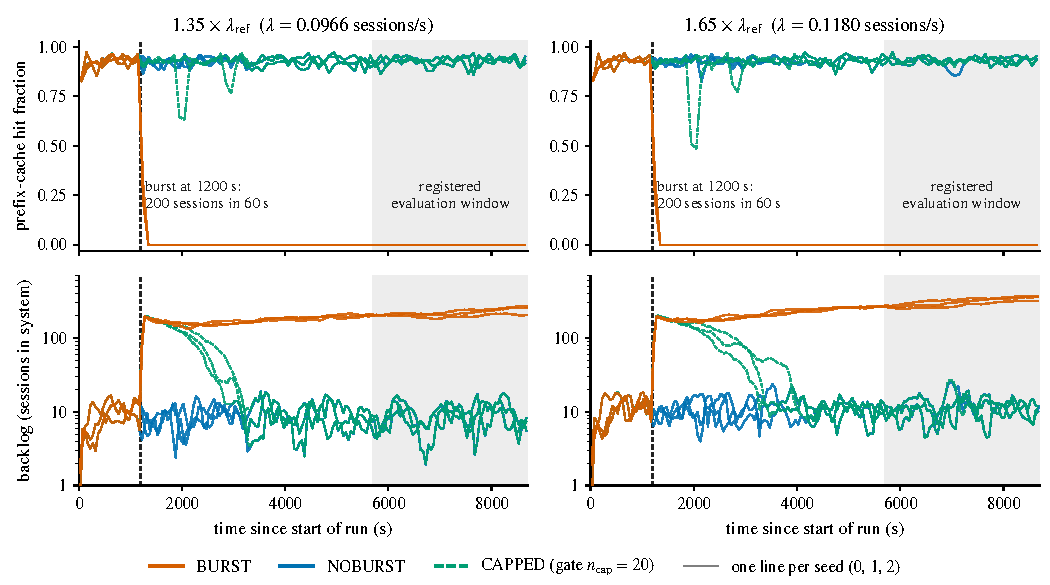
\includegraphics[width=\textwidth]{figs/fig1_e2_timeseries.pdf}
\caption{The trap on SGLang: the registered paired test E2 at nominal rates of 1.35~$\lref$ (left) and 1.65~$\lref$ (right),
$\lref=0.0715$\sps, the all-miss session rate measured with the radix cache disabled; one A100, a 300k-token KV pool. Top: hit fraction (turns with more than half of the prompt cached) in 100\,s
windows. Bottom: sessions in the system (log scale), including those in tool calls. One thin line per seed and arm. Dashed: a burst
of 200 sessions at 1200\,s. Shaded: the registered evaluation window. Without the burst (NOBURST) and with a client-side session cap
(CAPPED) the engine stays good; after it (BURST), every turn misses to the end of the run.}\label{fig:e2}
\end{figure*}

An LLM agent that calls tools sends its serving engine sessions of many turns: each prompt is the previous context plus the
output of the tool just run. Prefix caching keeps the key--value (KV) state of the previous turn, so a follow-up turn whose prefix
is still cached prefills only its new tokens~\citep{zheng2024sglang}. In our workload a hit prefills 551 tokens and a miss about
11{,}100, and a session's prefill work with every turn missing is about 16 times that with every follow-up hitting. The cached KV
belongs to sessions that sit idle in tool calls, and admitting waiting work evicts it. A burst of new sessions can therefore tip
the engine into a state in which every turn misses, the queue grows, the gap between a session's turns grows with it, and idle KV
is evicted before its owner returns. Fig.~\ref{fig:e2} shows this on SGLang: at loads that the engine carried from empty, a burst of
200 sessions left it at zero hits for the remaining 7500\,s.

\paragraph{What is not ours.} The phenomenon, its sustaining loop and a fluid model of its window are not new. Concurrently with
and independently of this work, Lu et al.\ showed on prefill--decode disaggregated SGLang with real agent traces that a finite surge
leaves the engine persistently degraded at a base load it previously sustained, identified the population--cache feedback that
sustains the failure, and modelled the vulnerable window with a fluid population balance and an empirical hit-rate
curve~\citep{lu2026cachetrap}. Their paper appeared first. The registered experiments of \S\ref{sec:evidence} up to SHED and TOOLSLOW were designed,
registered and run before it appeared (Appendix~\ref{app:timeline}); the theory of \S\ref{sec:trap} and the blind tests of
\S\ref{sec:validation} (TOOLSLOW-W, TOOLSLOW-D15 and CUT, registered on 2026-11-05) came afterwards, and the trap-state predictions
were made with Lu et al.'s paper in hand. The collapse is Denning's thrashing~\citep{denning1968thrashing}, a bad state that a feedback
loop sustains after its trigger is a metastable failure~\citep{bronson2021metastable,huang2022metastable}, and metastability from a
unimodal throughput curve, with bounded admission as the cure, is
classical~\citep{kleinrock1975aloha,carleial1975bistable,nelson1987stochastic}.

\paragraph{The question.} This paper asks what the trapped state \emph{is}. Quasi-static models treat it as the falling branch
of a throughput curve, $\dot n=\lambda-\mu(n)$; read literally in congestion, sessions then complete at the curve's low end and
accumulate at the excess over it. On our engines, where every trapped turn misses, both statements are wrong. Trapped runs
complete sessions faster than the all-miss capacity measured with caching disabled ($\lref$, the unit of every rate below), by up
to 2.4 times (one from-empty run at 6.5~$\lref$), while their backlog grows at about two thirds of the quasi-static rate. The gap matters to an operator: in model~F below, a cut to just below the throughput
measured in an all-miss trap does not clear it.

\paragraph{Contributions.}
\begin{enumerate}[label=(\arabic*),leftmargin=*]
\item \textbf{A renewal law for an idealized trap} (\S\ref{sec:trap}). We idealize the trapped engine as a fluid FIFO server on
which every turn misses and every turn rejoins the tail of the queue (model~F), analyse it exactly, and prove that along FIFO orbits
its cycles obey a linear renewal recursion (Theorem~\ref{thm:trap}). Below $\lmiss$ the trap drains, as is
classical; above it, the recursion's Perron root $z$ gives the convergence of every trapped state to a self-similar regime in which
the gap between a session's turns grows at $z-1$, the backlog at $\lambda(1-E[z^{-T}])$ and completions at $D=\lambda E[z^{-T}]$, with the turn mix tilted to
$G_kz^{-k}$. We decompose $D/\lmiss$ into a turn-count factor and a cost-growth factor, a youth premium above 1 for our workload
(Theorem~\ref{thm:premium}), and conclude that in model~F the throughput measured in a trap overstates the recovery threshold: only
$\lambda'<\lmiss$ drains it, after a busy period that diverges at the threshold (Corollary~\ref{cor:trapthr}). The self-similar
regime itself is known~\citep{khanin2001steady}, the recursion is a discrete renewal equation of Lotka--Leslie
type~\citep{feller1968introduction}, the critical case is the fluid counterpart of heavy-traffic state-space
collapse~\citep{reiman1988multiclass,dai1995multiclass}, and the premium has a processor-sharing
analogue~\citep{jeanmarie1994transient}. What we add, as far as a targeted search found, is the derivation of that recursion along
FIFO orbits, which carries every trapped state into the regime with an exact virtual origin, and the turn-count and cost-growth
factors of the premium. Corollary~\ref{cor:trapthr} is the operational reading of Theorem~\ref{thm:premium} with the classical drain
condition; what is new about it is its test on the engine.
\item \textbf{A test of the theory across engines} (\S\ref{sec:validation}). With no parameter fitted to any trap measurement, model~F
matches, across 57 stuck runs on SGLang and vLLM, two GPUs and two models (36 of them from registered protocols, on 30 distinct
arrival plans), the trapped turn mix (within 3\% in 50 of them), the pooled linear growth of the gap (median ratio of measured to
predicted slope 1.01; per run 0.04--1.81) and completions above the all-miss capacity (in every run). It also explains, post hoc,
why our registered trap rule was fragile at the lower rate. These checks are retrospective. Three blind tests followed, with
predictions frozen before the runs existed; they are blind in outcome, and the tolerances of the trap-state scores were set on the
earlier runs. A pre-registered 30\,s tool slowdown lasting 1800\,s with no burst, designed after a 900\,s one had trapped 1 of 3,
trapped the engine in 3 of 3 runs while their paired no-burst runs stayed good, and on these runs, in one cell whose outcome every
frozen model predicted, the theory met all four pooled scores. A second slowdown, at 1.65~$\lref$, chosen so that our two frozen
predictors disagree, trapped 1 of 3 runs, as the calibrated simulator had predicted seed by seed, against the first-principles
model's plan-averaged TRAPS. After a burst, a cut in arrivals to below the trapped throughput of the same seeds' uncut runs, but
above the all-miss capacity, left all three CUT-A runs trapped, and a cut below the all-miss capacity drained the three CUT-B traps
only slowly, all still stuck 6300\,s after the cut, as model~F predicted. Each arm's registered rule rejected the naive reading, and
CUT-A's also the quasi-static one, but not intermediate readings (a flat backlog fits CUT-A as well over $[3000,8700)$\,s); what
singles out model~F against them is post hoc: CUT-A's late-window slopes and CUT-B's completions below the all-miss capacity.
\item \textbf{A first-principles account of entry} (\S\ref{sec:entry}). We derive the closed-population throughput curve $\mu(n)$ from
the pool, the workload and a cost model fitted to server-log timing only. Its all-miss onset is the sessions in tool calls plus one
pool of running sessions, which a faster GPU moves out, and we report its out-of-sample record, misses included. Against a post-hoc
reading of Lu et al.'s concurrent model on our colocated cells, with one hit curve fitted on one cell (they built the model for
disaggregated serving and do not use the curve to predict hits), the measured cliff moved out on the H200, by 6.7 and 10.9 sessions
at the two pools against 5.8 and 6.6 from the tool-call term, and on the five cells frozen before their runs were read our crossings err by 1.5 sessions on average, against 4.1.
\item \textbf{Control as two exits} (\S\ref{sec:control}). In model~F, starving the trap needs $\lambda'<\lmiss$, and on the engine a
registered cut to 0.85~$\lref$ drained it only slowly (CUT-B); refusing arrivals (SHED) sheds sessions: in a registered test a 3600\,s stop drained the trap and refused 355--378 sessions. Restoring reuse with a
session cap, which leaves model~F, does not: in registered tests the cap rescued 9 of 9 established zero-hit traps at the same
offered load without shedding a session, at a price of 386--569\,s of waiting at the client per paused session and 45--97\% of the
goodput of the hour after the burst, and the engine stayed good after the cap was removed.
\item \textbf{A registered evidence base} (\S\ref{sec:evidence}): paired tests with matched no-burst and capped arms on common random
numbers on two engines, two GPUs and two models, a seed-replicated bracket of the basin in burst size, and registered negatives.
\end{enumerate}

\noindent Model~F is an idealization, and we do not prove that the engine converges to it. Sessions are synthetic (exponential
5\,s tool times, no shared prefixes) and the models are dense and 7--8B in size. Section~\ref{sec:related} positions the work in
detail.
